\section{Εισαγωγή}
\pSpace Η ανάπτυξη της εφαρμογής ακολούθησε το πακέτο \e{MEAN}, το οποίο αναφέρεται στο \e{MongoDB}, \e{ExpressJS}, \e{Angular} και \e{NodeJS}.Σε αυτά προσθέτηκαν το \e{Socket.io}, \e{RxJS} και την πρώτη έκδοση του \e{Google Material Design} σε ενα \e{framework} λεγόμενος \e{Angular Material 2}. Οι τεχνολογίες \e{HTMl, CSS} και \e{JavaScript} οι οποίες είναι απαραίτητες για την κατασεύη μιας διαδικτυακής εφαρμογής δεν αναφέρθηκαν λόγω του ότι θεωρήθηκαν αυτονόητα, και δεν χρειάζονται περαιτέρων εξηγήσεις.

\section{\e{NodeJS}}
\pSpace Το \e{Node.js®} είναι ένα \e{JavaScript runtime} που βασίζεται στη μηχανή \e{JavaScript V8} του \e{Chrome}. Το \e{Node.js} χρησιμοποιεί ένα \e{event-driven, non-blocking} μοντέλο I/O, το οποίο το καθιστά ελαφρύ και αποδοτικό. Στόχος του \e{Node} είναι να παρέχει ένα εύκολο τρόπο δημιουργίας κλιμακωτών διαδικτυακών εφαρμογών. 
\e{\parencite{nodejs}}

\subsection*{Γιατί}
\pSpace Σε αντίθεση από τα περισσότερα σύγχρονα περιβάλλοντα ανάπτυξης εφαρμογών δικτύων μία διεργασία \e{Node} δεν στηρίζεται στην πολυνηματικότητα αλλά σε ένα μοντέλο ασύγχρονης επικοινωνίας εισόδου/εξόδου. Το \e{HTTP} στο \e{Node} είναι σχεδιασμένο για συνεχή μετάδοση και χαμηλό χρόνο καθυστέρησης. Αυτό καθιστά το \e{Node} κατάλληλο για τη δημιουργία μιας \e{web library} ή ενός \e{framework}. Επίσης στο \e{Node} σχεδόν καμία λειτουργία δεν εκτελεί απευθείας I/O, οπότε η διαδικασία δεν μπλοκάρει ποτέ.
\e{\parencite{nodejs}}

\subsection*{\e{Node Package Manger}}
\pSpace Το οικοσύστημα πακέτων \e{Node.js, npm,} είναι το μεγαλύτερο οικοσύστημα βιβλιοθηκών ανοικτού κώδικα στον κόσμο.Η κοινότητα έχει δημιουργήσει ένα ολόκληρο οικοσύστημα από βιβλιοθήκες που προορίζονται ή είναι συμβατές με το \e{Node}. Ανάμεσά τους εργαλεία που ξεχώρισαν όπως το \e{node-mysql}, το \e{Mongodb} και το \e{Express} παίζουν σημαντικό ρόλο υποστηρίζοντας την ασύγχρονη διάδραση με τις παραδοσιακές και \e{NoSQL} μεθόδους βάσεων δεδομένων. Αυτό επιτυγχάνεται με την χρήση του \e{node package manager} το οποίο επιτρέπει την εγκατάσταση των παραπάνω βιβλιοθηκών. Χρησιμοποιείται συνήθως σε εφαρμογές \e{Chat, Proxy, Http Server} καθώς και για παρακολούθηση εφαρμογών του συστήματος \e{(monitoring)}
\e{\parencite{nodejs_wikipedia}}. Για την χρήση του \e{npm} πρέπει να δημιουργηθεί ένα αρχείο με το όνομα \e{project.json} στον φάκελο της εφαρμογής. Σε αυτό το αρχείο αποθυκεύονται τα στοιχεία της εφαρμογής με την χρήση της εντολής: \selectlanguage{english}
    \begin{lstlisting}[language=command.com]
    $\dollar$ npm init
    \end{lstlisting}
    \selectlanguage{greek} Για την εγκατάσταση πακέτων χρησημοποίητε η εντολή: 
    \selectlanguage{english}
    \begin{lstlisting}[language=command.com]
    $\dollar$ npm install "package_name" --save
    \end{lstlisting}
    \selectlanguage{greek} Για την χρήση πακέτων μόνο για το \e{development} στάδιο προστίθετε η επιλογή \e{"-dev"} στο τέλος της εντολής. Τα αρχεία όλων των πακέτων αποθυκεύονται σε έναν φάκελο με το όνομα \e{node\_modules}. Αν κάποιος έχει το αρχείο \e{project.json} μπορεί με την εντολή:
    \selectlanguage{english}
    \begin{lstlisting}[language=command.com]
    $\dollar$ npm install
    \end{lstlisting}
    \selectlanguage{greek} να κατεβάσει όλα τα πακέτα που χρειάζεται η εφαρμογή.
 
\subsection*{Εγκατάσταση}
\pSpace Για να εγκαταστήσει κανείς το \e{Node.js} στον υπολογιστή του, το μόνο που μένει να κάνει είναι να κατεβάσει την έκδοση που τον βολεύει απο την ιστοσελίδα \newline\e{https://nodejs.org/en/download/} και να την εγκαταστήσει. 

\subsection*{Αλλες επιλογές}
\pSpace Το \e{Node} είναι παρόμοιο στο σχεδιασμό και επηρεάζεται από συστήματα όπως το \e{Event Machine} της \e{Ruby} και το \e{Twisted} της \e{Python}.
\e{\parencite{nodejs}}

\section{\e{ExpressJS}}
\pSpace Το \e{Express} είναι ένα μικρό και ευέλικτο \e{Node.js web application framework} που παρέχει ένα ισχυρό σύνολο λειτουργιών για \e{web} και κινητές εφαρμογές. Παρέχει ένα λεπτό στρώμα θεμελιωδών χαρακτηριστικών εφαρμογών ιστού.
\e{\parencite{express}}

\subsection*{Γιατί}
\pSpace Χρησιμοποιήσαμε το \e{Express} γιατί το \e{Node} δεν είχε έτοιμο \e{http routing} και έπρεπε να το γράψουμε εμείς. Ωπότε διαλέξαμε να εγκαταστήσουμε το \e{Express} που μας παρέχει αυτή την λειτουργία. 

\subsection*{Πλεονεκτήματα}
\pSpace Το \e{Express} μας παρέχει μια μεγάλη γκάμα λειτουργιών για το \e{http routing} όπως:
\begin{itemize}
    \item \e{Route methods:}
        Οι μέθοδοι διαδρομής προέρχονται από μια από τις μεθόδους \e{HTTP} π.χ. \e{get,post,} κ.α. και συνδέονται με ένα \e{instance} της κλάσης \e{express}.
    \item \e{Route paths - regular expression:}
        Οι διαδρομές διαδρομής, σε συνδυασμό με μια \e{request} μέθοδο, καθορίζουν τα τελικά σημεία στα οποία μπορούν να γίνουν \e{requests}. Οι διαδρομές διαδρομής μπορούν να είναι συμβολοσειρές, μοτίβα συμβολοσειρών ή κανονικές εκφράσεις.
    \item \e{Route parameters:}
        Οι παράμετροι διαδρομής είναι ονομαστά τμήματα \e{URL} που χρησιμοποιούνται για την καταγραφή των τιμών που καθορίζονται στη θέση τους στη διεύθυνση \e{URL}.
    \item \e{Route handlers:}
        Οι διαχειριστές δρομολογίων μας δίνουν την δυνατότητα να προωθήσουμε το \e{request} σε όσες διαδρομές θέλουμε. Πρέπει να προσέχουμε πολύ όμως το \e{request} να έχει το μέγιστο ένα \e{response} σε όλη την διάρκεια των διαδρομών του.
    \item \e{Response methods:}
        Οι μέθοδοι απόκρισης στέλνουν μια απάντηση στον πελάτη και τερματίζουν τον κύκλο απόκρισης αιτήματος. Αν δεν καλέσουμε καμία μέθοδο απόκρισης τότε το αίτημα του πελάτη θα παραμείνει κρεμασμένο.
\end{itemize}
\e{\parencite{express_routing}}
 
\subsection*{Εγκατάσταση}
\pSpace Για την εγκατάσταση του \e{Express} εκτελούμε την εντολή:
    \selectlanguage{english}
    \begin{lstlisting}[language=command.com]
    $\dollar$ npm install express --save
    \end{lstlisting}
    \selectlanguage{greek}

\subsection*{Αλλες επιλογές}
\pSpace Μια διάσημη άλλες επιλογή είναι το \e{Hapi} \e{\parencite{colorlib_ivanovs}}. Το \e{Hapi} είναι ένα πλούσιο σε λειτουργίες \e{framework} το οποίο ευνοεί το \e{configuration} και προσπαθεί να καλύψει έναν ευρύτερο φάσμα χρήσεων. Αρχικά δημιουργήθηκε από ένα μέλος της \e{WalmartLabs} και προορίζεται για μεγάλες ομάδες και μεγάλα έργα. Εξαιτίας αυτού, μπορεί να είναι λίγο βαρύ για μικρά έργα \e{\parencite{hapi_vs_express}}. Θα μπορούσαμε να χρησιμοποιήσουμε \e{Locomotive, Compound}.


\section{\e{Socket.io}}
\pSpace Το \e{Socket.IO} είναι μια βιβλιοθήκη \e{JavaScript} για εφαρμογές \e{web} σε πραγματικό χρόνο. Επιτρέπει την αμφίδρομη επικοινωνία σε πραγματικό χρόνο, μεταξύ των \e{web clients} και των διακομιστών. Έχει δύο μέρη: μια βιβλιοθήκη πελάτη που τρέχει στο πρόγραμμα περιήγησης, και μια βιβλιοθήκη διακομιστή για \e{Node.js}. Και τα δύο συστατικά έχουν σχεδόν ταυτόσημο \e{API}. Τα τμήματα διαπραγμάτευσης πρωτοκόλλου προκαλούν σε έναν πελάτη που υποστηρίζει το τυπικό \e{WebSocket} να μην μπορεί να επικοινωνήσει με ένα διακομιστή \e{Socket.IO}. Και ένας υπολογιστής-πελάτης υλοποίησης \e{Socket.IO} δεν μπορεί να μιλήσει με διακομιστή \e{WebSocket} ή \e{Long Polling Comet} που δεν βασίζεται σε \e{Socket.IO}. Αυτό συμβαίνει γιατί το \e{Socket.IO} δεν είναι μια βιβλιοθήκη \e{WebSocket} με εναλλακτικές επιλογές σε άλλα πρωτόκολλα σε πραγματικό χρόνο. Πρόκειται για μια \e{custom} υλοποίηση πρωτοκόλλου μεταφοράς σε πραγματικό χρόνο, πάνω από άλλα πρωτόκολλα σε πραγματικό χρόνο. Επομένως, το \e{Socket.IO} απαιτεί τη χρήση των βιβλιοθηκών \e{Socket.IO} και από πλευράς πελάτη και διακομιστή. Το \e{Socket.IO} χειρίζεται τη σύνδεση με διαφάνεια και θα γίνει αυτόματη αναβάθμιση στο \e{WebSocket} αν είναι δυνατόν \e{\parencite{socket-io_wikipedia}}. Το \e{Socket.IO} επιτρέπει την αμφίδρομη επικοινωνία βασισμένη σε γεγονότα σε πραγματικό χρόνο.Λειτουργεί σε κάθε πλατφόρμα, πρόγραμμα περιήγησης ή συσκευή, εστιάζοντας εξίσου στην αξιοπιστία και την ταχύτητα \e{\parencite{socket-io}}.

\subsection*{Γιατί}
\pSpace Το \e{Socket.IO} παρέχει ένα αμφίδρομο κανάλι επικοινωνίας μεταξύ ενός πελάτη και ενός διακομιστή. Αυτό σημαίνει ότι ο διακομιστής μπορεί να στείλει μηνύματα στους πελάτες. Για αυτό χρησιμοποιήσαμε το \e{Socket.IO} για την χρήση \e{real time} δεδομένων, καίρια για την λειτουργία της εφαρμογής όπως \e{task dependencies}, chat κ.α. 

\subsection*{Εγκατάσταση}
\pSpace Το \e{Socket.IO} απο αποτελείται απο δύο κομμάτια. Το \e{client} και το \e{server}. Για την εγκατάσταση του \e{server} εκτελούμαι την εντολή:
\selectlanguage{english}
    \begin{lstlisting}[language=command.com]
    $\dollar$ npm install socket.io --save
    \end{lstlisting}
    \selectlanguage{greek}
Και για την εγκατάσταση του \e{client} εκτελούμαι την εντολή:
\selectlanguage{english}
    \begin{lstlisting}[language=command.com]
    $\dollar$ npm install socket.io-client --save
    \end{lstlisting}
    \selectlanguage{greek}

\subsection*{Αλλες επιλογές}
\pSpace Τα \e{WebSockets} είναι μια προηγμένη τεχνολογία που καθιστά δυνατό το άνοιγμα μιας αλληλεπιδραστικής περιόδου επικοινωνίας μεταξύ του προγράμματος περιήγησης του χρήστη και ενός διακομιστή. Άλλες \e{javascript} βιβλιοθήκες που χρησιμοποιούν \e{WebSockets} για το \e{Node.js} είναι: μ\e{WebSockets, SocketCluster, Total.js, Faye} και \e{ws}
\e{\parencite{mozilla_developer}}.

\section{\e{MongoDB}}
\pSpace Η \e{MongoDB} είναι μία \e{open-source NoSql} βάση δεδομένων. Σκοπός της είναι να συνδυάσει την πλούσια λειτουργικότητα των σχεσιακών βάσεων δεοδομένων με την ταχήτητα και επεκτασιμότητα που έχουν τα δεδομένα του τύπου κλειδί-τιμή \e{(key-value)}. Πρωτοαναπτύχθηκε το 2007 απο την εταιρεία \e{10gen} ως μέρος μιας πλατφόρμας ως προϊόν εξυπηρέτησης. Το 2009 η εταιρεία μετατοπίστηκε σε ένα μοντέλο ανάπτυξης ανοιχτού κώδικα, με την εταιρεία να προσφέρει εμπορική υποστήριξη και άλλες υπηρεσίες. Η \e{MongoDB} εκδόθηκε σε συνδυασμό της Γενικής Δημόσιας Άδειας \e{GNU Affero} και της Άδειας \e{Apache}. Η εταιρεία \e{10gen} άλλαξε το όνομα της σε \e{MongoDB Inc.} το 2013. 

\subsection*{Αποθύκευση δεδομένων}
\pSpace Αντί για πίνακες, στήλες και γραμμές η \e{MongoDB} χρησιμοποιεί συλλογές και έγγραφα. Οι συλλογές είναι κάτι αντίστοιχο των πινάκων. Τα έγγραφα είναι μια εγγραφή σε μια συλλογή, τα οποία αποτελούνται απο ζευγάρια πεδίων και τιμών. Η μορφή των εγγράφων μοιάζουν πολύ με αντικείμενα \e{JSON} και η \e{MongoDB} δίνει την δυνατότητα στα στοιχεία κάθε εγγράφου να διαφέρουν μεταξύ τους. Η δομή των δεδομένων είναι ευέλικτη και μπορεί αλλαχτεί πολύ εύκολα, οποιαδήποτε στιγμή. Οι τιμές των πεδίων μπορεί να περιέχουν άλλα έγγραφα, πίνακες \e{(arrays)}, ακόμα και πίνακες \e{(arrays)} εγγράφων.

\subsection*{Γιατί}
\quad Διαλέξαμε να χρησιμοποιήσουμε την \e{MongoDB} γιατί είναι μια γρήγορη και ευέλικτη βάση δεδομένων. Υποστηρίζει μια γλώσσα πλούσια σε ερωτήματα για λειτουργίες \e{CRUD}, πρόσμιξη δεδομένων \e{(data} aggregation), αναζήτηση κειμένου και γεωχωρικά ερωτήματα \e{(geospatial queries)}. Η δυνατότητα χρήσης ενός δυναμικού σχήματος \e{(schema)} μας επιτρέπει να αλλάζουμε την δομή των δεδομένων που αποθυκεύουμε αλλά και αυτών που έχουν ήδη αποθυκευτεί πολύ εύκολα. Επίσης η επεκτασιμότητα της μας βοήθησε παρα πολύ στο να επεκτείνουμε και ολόκληρη την εφαρμογή προσθέτοντας πράγματα τα οποία δεν είχαμε υπολογίσει εξαρχής.
 
\subsection*{Πλεονεκτήματα}
\quad Κάποια απο τα πλεονεκτήματα της \e{MongoDB} είναι, η υπηρεσία λειτουργίας αντιγράφων της βάσης, η οποία παρέχει αυτόματη ανάκαμψη από βλάβες και πλεονασμό δεδομένων. Τα ενσωματωμένα έγγραφα και πίνακες μειώνουν την ανάγκη για δαπανηρές πράξεις τύπου \e{join} και την χρήση I/O της βάσης. Οι δείκτες μπορούν να δεικτοδοτήσουν κλειδιά και σε ενσωματωμένα έγγραφα. Τα έγγραφα αντιστοιχούν σε φυσικούς \e{(native)} τύπους δεδομένων πολλών προγραμματιστικών γλωσσών, διευκολύνοντας πολύ τον προγραμματισμό εφαρμογών.

\subsection*{Εγκατάσταση}
\quad Για την εγκατάσταση της \e{MongoDB} ακολουθήσαμε τα εξής βήματα.
Τα παρακάτω βήματα είναι για το \e{server} κομμάτι της εφαρμογής.
\begin{itemize}
    \item Κατεβάσαμε και εγκαταστήσαμε την τελευταία \e{community server} έκδοση 
    για \e{windows} απο την σελίδα \e{"https://www.mongodb.com/download-center\#community"}
    \item Δημιουργήσαμε έναν φάκελο με όνομα \e{"data"} στο \e{path "C:{\textbackslash}data".} 
    Εδώ θα αποθεύονται όλα τα απαραίτητα αρχεία για την λειρουργία της \e{MongoDB}.
    \item Τρέξαμε το αρχείο \e{"mongod.exe"} το οποίο ξεκινά την βάση.
    \item Αυτό το βήμα είναι για την εγκατάσταση των απαραίτητων \e{driver} για να χρησιμοποιήσουμε την \e{MongoDB} μέσω του \e{server} \e{ NodeJs.} Δημιουργήσαμε ένα αρχείο με όνομα \e{"package.json"} στον φάκελο της εφαρμογής μας και εκτελέσαμε της εξής εντολές μέσω \e{cmd} στον ίδιο φάκελο.
    \selectlanguage{english}
    \begin{lstlisting}[language=command.com]
    $\dollar$ npm init
    $\dollar$ npm install mongodb --save
    \end{lstlisting}
    \selectlanguage{greek}
    Η εντολή \e{"npm init"} χρησιμοποιήθηκε για να φορτωθούν στο αρχείο \e{"package.json"} οι απαραίτητες ρυθμίσεις της εφαρμογής. 
    Η εντολή \e{"npm install mongodb --save"} εγκαθιστά τους απαραίτητους \e{driver} για να συνδεθούμαι με την βάση απο τον \e{server.} Η εντολή \e{--save (option)} αποθυκεύει στο αρχείο \e{"package.json"} τις απαραίτητες πληροφορίες ότι έχουμε εγκαταστήσει και ότι θα χρειαστούμαι τους \e{driver} που μόλις κατεβάσαμε. Τα αρχεία που κατεβάσαμε έχουν αποθυκευτεί σε έναν φάκελο με το όνομα \e{"node\_modules"} στον φάκελο τον οποίο βρισκόμαστε.
\end{itemize}

\subsection*{Αλλες επιλογές}
\quad Υπάρχουν πολλές βάσεις δεδομένων που θα μπορούσαμε να είχαμε χρησιμοποιήσει αντί για την \e{MongoDB}. Αν μιλάμε όμως μόνο για \e{NoSQL} βάσεις που λειτουργούν με έγγραφα τότε οι επιλογές μας ήταν μια απο αυτές: \e{Apache CouchDB, ArangoDB, Clusterpoint, Couchbase, Cosmos DB, HyperDex, IBM Domino, MarkLogic, MongoDB, OrientDB, Qizx, RethinkDB.}

\section{\e{Angular}}
\quad \e{Angular} είναι ένα \e{Front-end JavaScript framework} το οποίο διευκολύνει την κατασκεύη των \e{web} εφαρμογών. Παρέχει μια σειρά από λειτουργίες που καθιστούν τετριμμένη την εφαρμογή των σύνθετων απαιτήσεων των σύγχρονων εφαρμογών. Συνδυάζει πρακτικές όπως \e{dependency injection, end-to-end tooling} και \e{declarative templates} για να πετύχει ο προγραμματιστής την βέλτιστη λύση.\par
Αυτή η πλατφόρμα πέρασε μια πλήρης επανεγγραφή σε σχέση με την προηγούμενη έκδοση , \e{AngularJS}, προσθέτωντας πολλά νέα μοναδικά χαρακτηριστικά. 


\subsection*{Γιατί}
\quad Έναν απο τους βασικότερους λόγους που επιλέξαμε αυτό το \e{framework} , είναι το υπερσύνολο του \e{JavaScript}, το λεγόμενο \e{TypeScript}. Αυτό φέρνει τις έννοιες του  \e{ OOP (Object-Oriented Programming), Static Typing} και \e{Generics} στον χώρο των ιστοσελίδων και επιπλέον <<αναγκάζει>> τον προγραμματιστή να γράψει σωστότερο κώδικα.
To \e{TypeScript} είναι συμβατό και με την παλιά έκδοση \e{ES5 - JavaScript} , συμπεριλαμβάνοντας τα πλεονεκτήματα του \e{ES6}, όπως \e{Lambda expressions, Iterators}, βρόχοι \e{For/of} και \e{Reflection}.\par Επιπλέον , οι εφαρμογές \e{Angular} ακολουθούν την έννοια του \e{Single Page Application-SPA}, πράγμα που σημαίνει πως η δικτυακή εφαρμογή φορτώνει μόνο στην αρχή τα απαραίτητα \e{HTML, CSS, JavaScript}, ύστερα αλλάζοντας μόνο το περιεχόμενο με κάθε αλληλεπίδραση του χρήστη.\par Επιπροσθέτως, μια σημαντική μοναδική λειτουργία της παρούσας πλατφόρμας, είναι το \e{AoT - Ahead Of Time Compilation}, το οποίο μεταγλωτίζει όλα τα αρχεία σε κώδικα \e{JavaScript}, στην φάση της τελικής κατασκευής. Αυτό έχει ως αποτέλεσμα,  το πρόγραμμα περιήγησης του χρήστη να κατεβάζει ένα αρχείο μόνο, βελτιώνοντας κατά μεγάλο ποσοστό την απόδοση.\par Επίσης, η υποστήριξη της \e{Google}, η μεγάλη κοινότητα εταιριών και προγραμματιστών που χρησιμοποιούν αυτήν την πλατφόρμα, είναι ένα πολύ σημαντικό προσόν, το οποίο στην διάρκεια της ανάπτυξης, αποδεικνύεται κρίσιμο.\par
Ακόμη αξίζει να σημειωθούν οι σημαντικότερες διαφορές μεταξύ \e{Angular 2/4/5} με \e{AngularJS}:
\begin{itemize}
    \item Η κύρια αρχιτεκτονική του βασίζεται σε μια ιεραρχία από \e{Components} σε σχέση με τα \e{Scopes} και \e{Controllers} της αρχικής έκδοσης
    \item Χρησιμοποιεί μια διαφορετική συντακτική , έχοντας τα <<[ ]>> για την δέσμευση ιδιότητας και <<( )>> για την δέσμευση συμβάντων
    \item Η ανάπτυξη είναι ευκολότερη εφόσον τα θέματα περί της κινητής απόδοσης , αντιμετωπίζονται πρώτα
    \item \e{Modularity} - Πολλές απο τις βασικές λειτουργίες έχουν χωριστεί σε \e{modules} (ενότητες), παράγοντας έτσι έναν γρηγορότερο και ελαφρύτερο πυρήνα
    \item Υποστήριξη μόνο στα σύγχρονα προγράμματα περιήγησης - μειώνει την ανάγκη αντιμετώπισης συμβατότητας με τις παλιές εκδόσεις των \e{Browser}
    \item Δυναμική φόρτωση
    \item \e{Asynchronous template compilation}
    \item Απλούστερη δρομολόγηση
    \item Υποστήριξη αντιδραστικού προγραμματισμού (\e{Reactive Programming}) με χρήση \e{RxJS} 
\end{itemize}

\subsection*{Εγκατάσταση}
\quad Η εγκατάσταση του \e{framework}, απαιτεί την ύπαρξη του \e{NodeJS} και \e{NPM-Node Package Manager} στο σύστημα. Η επαλήθευση αυτού του πράγματος, γίνεται με δύο απλές εντολές από το περιβάλλον του \e{Terminal}:

\selectlanguage{english}
\begin{lstlisting}[language=command.com]
  $\dollar$ node -v
  $\dollar$ npm -v
\end{lstlisting}
\selectlanguage{greek}

Αφού υπάρχουν τα δύο προαπαιτούμενα, η επόμενη εντολή θα εγκαταστήσει παγκοσμίως το \e{Angular CLI}

\selectlanguage{english}
\begin{lstlisting}[language=command.com]
$\dollar$ npm install @angular/cli -g
\end{lstlisting}
\selectlanguage{greek}

Έχοντας εγκαταστήσει επιτυχής όλα τα παραπάνω, η δημιουργία ενός \e{Demo} έργου φαίνεται στα επόμενα βήματα:

\begin{enumerate}[label=\textbf{\arabic*}]
   \item 
   \selectlanguage{english}
	\begin{lstlisting}[language=command.com]
	$\dollar$ ng new my-new-app
	\end{lstlisting}
    \selectlanguage{greek}
    
    Αυτή η εντολή δημιουργεί ενα καινούργιο \e{project} με το όνομα \e{my-new-app}, συμπεριλαμβάνοντας τα βασικά \e{Dependencies}  στο τρέχον κατάλογο.
  \item 
   \selectlanguage{english}
   \begin{lstlisting}[language=command.com]
    $\dollar$ cd my-new-app
    $\dollar$ ng serve --open
    \end{lstlisting}
    \selectlanguage{greek}    
    Πηγαίνει στον κατάλογο \e{my-new-app} ,ξεκινάει τον \e{Server} και ανοίγει στο προεπιλεγμένο πρόγραμμα περιήγησης, το έργο. Κάθε αλλαγή και αποθήκευση στα αρχεία του, φαίνεται αμέσως στο \e{Browser}.
\end{enumerate}
% Η εγκατασταση σε ενα μεγαλυτερο προτζεκτ , χρειαζεται βεβαιως περισσοτερα βηματα... package.json κλπ κλπ

\subsection*{Αλλες επιλογές}
Οι σημερινές απαιτήσεις εφαρμογών οδήγησαν τους προγραμματιστές να εστιάσουν την προσοχή τους στα έτοιμα \e{Frameworks} για 3 κύριους λόγους : 
\begin{itemize}
    \item Αποτελεσματικότητα - Τα έργα που χρειάζονταν κανονικά μήνες, χιλιάδες γραμμές κώδικα και αρκετούς πονοκεφάλους, μπορούν να επιτευχθούν πολύ ταχύτερα με καλά δομημένα πρότυπα και λειτουργίες. Επίσης οι ομάδες συννενοούνται ευκολότερα.
    \item Ασφάλεια - Τα κορυφαία \e{framework} έχουν σταθερές ρυθμίσεις ασφαλείας και υποστηρίζονται από μεγάλες κοινότητες όπου τα μέλη και οι χρήστες λειτουργούν επίσης ως δοκιμαστές
    \item Κόστος - Τα περισσότερα είναι ανοικτού κώδικα , δωρεάν και καθώς είναι πιο αποτελεσματικά, μειώνεται ο χρόνος για την δημιουργία της εφαρμογής αρά και η τελική τιμή
\end{itemize}
Όπως προκύπτει και από Σχ. \ref{fig:jsComparison}, οι κυριότερες λύσεις είναι πέντε:
\begin{itemize}
    \item \e{Angular}
    \item \e{React}
    \item \e{Ember}
    \item \e{Vue}
    \item \e{Backbone}
\end{itemize}
\begin{figure}[ht]
\centering
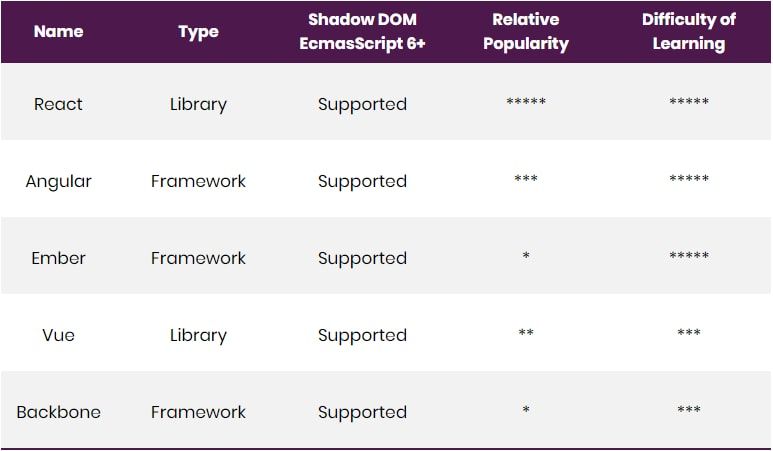
\includegraphics[scale=0.5]{images/comparisonJSFW.jpg}
\caption{Σύγκριση ανάμεσα στα 5 πιο διαδεδομένα \e{frameworks \parencite{javascriptComparison}}}
\label{fig:jsComparison}
\end{figure}
\quad Παρατηρείται πως τα δύο από αυτά θεωρούνται βιβλιοθήκες. Στην πραγματικότητα όμως η χρησιμότητα και τα χαρακτηριστικά που προσφέρουν μοιάζουν πιο πολύ με ένα σύγχρονο \e{framework}.\par
Η επιλογή ενός για τη δημιουργία μελλοντικού έργου, εξαρτάται από τη περιπλοκότητα και τις απαιτήσεις. Για παράδειγμα, το \e{Angular} θεωρείται από τους περισσότερους ιδανικό για τα μεγαλύτερα και πιο περίπλοκα έργα, γιατί τότε θα προσφέρει τα αποτελέσματα που επιθυμούνται. Σε αντίθεση με \e{React, Vue} η ταχύτητα/αποτελεσματικότητα είναι πολύ μειωμένη στα συνηθισμένα μικρά \e{project}. Επίσης απαιτεί απο τους προγραμματιστές περισσότερες γνώσεις και η καμπύλη εκμάθησης είναι απότομη (\e{learning-curve}-Σχ.\ref{fig:angular_vue_react_learning_curve}).
\begin{figure}[ht]
\centering
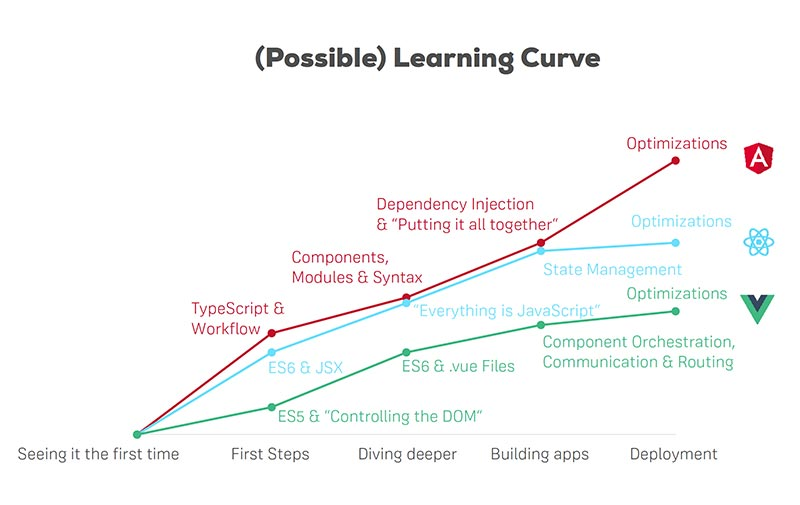
\includegraphics[scale=0.3]{images/angular-react-vue-learning-curve.jpg}
\caption{Κάμπυλη εκμάθησης ανάμεσα σε \e{Angular, React} και \e{Vue frameworks \parencite{angular_vue_react_learning_curve}}}.
\label{fig:angular_vue_react_learning_curve}
\end{figure}

\section{\e{RxJS}}
\quad Μια άλλη τεχνολογία που χρησιμοποιήθηκε στην υλοποίηση του έργου της παρούσας πτυχιακής, είναι το \e{RxJS}. Υπό την μορφή μιας βιβλιοθήκης γραμμένη σε \e{JavaScript} με υποστήριξη του \e{TypeScript}, φέρνει την έννοια του αντιδραστικού προγραμματισμού στον ιστό. Αυτό σημαίνει πως η εφαρμογή <<αντιδρά>> στις αλλαγές που συμβαίνουν όπως γεγονότα με επίδραση του χρήστη, λήψη δεδομένων κλπ.

\subsection*{Τι είναι}
\quad Ο αντιδραστικός προγραμματισμός (\e{Reactive Programming}), είναι ένα ασύγχρονο πρότυπο προγραμματισμού που αφορά τις ροές δεδομένων και την διαδόση της αλλαγής. Αυτό σημαίνει ότι είναι δυνατή η εύκολη έκφραση στατικών (π.χ. πίνακες) ή δυναμικών (π.χ.γεγονότα) ροών δεδομένων μέσω της χρησιμοποιούμενης γλώσσας προγραμματισμού, και ότι υπάρχει υποθετική εξάρτηση στο σχετικό μοντέλο εκτέλεσης. Πράγμα που διευκολύνει την αυτόματη διάδοση της αλλαγής που σχετίζεται με τη έν λόγο ροή.
Ο ορισμός αυτού του τύπου προγραμματισμού, το δίνει ο γάλλος \e{Gérard Berry} σε μια ερευνητική του έκθεση πάνω σε αυτό το θέμα \e{\parencite{real_time_programming_gerard}}:
\blockquote{Είναι βολικό να διακρίνει κανείς περίπου τρία είδη προγραμμάτων. Τα προγράμματα μετασχηματισμού υπολογίζουν τα αποτελέσματα από ένα δεδομένο σύνολο εισόδων: Τυπικά παραδείγματα είναι οι μεταγλωττιστές ή τα προγράμματα αριθμητικών υπολογισμών.Τα αλληλεπιδραστικά προγράμματα αλληλεπιδρούν με δικό τους ρυθμό και ταχύτητα, με τους χρήστες ή άλλα προγράμματα: Από την άποψη του χρήστη, ένα σύστημα \e{Time-Sharing} είναι διαδραστικό. Τα αντιδραστικά προγράμματα διατηρούν επίσης μια συνεχή αλληλεπίδραση με το περιβάλλον τους, αλλά με ταχύτητα που καθορίζεται από το περιβάλλον, όχι από το ίδιο το πρόγραμμα. Τα διαδραστικά προγράμματα λειτουργούν με το δικό τους ρυθμό και ασχολούνται κυρίως με την επικοινωνία, ενώ τα αντιδραστικά προγράμματα λειτουργούν μόνο ως απάντηση στις εξωτερικές απαιτήσεις και συνήθως ασχολούνται με τον ακριβή χειρισμό διακοπών. Τα προγράμματα Πραγματικού Χρόνου είναι συνήθως αντιδραστικά. Ωστόσο, υπάρχουν αντιδραστικά προγράμματα που συνήθως δεν θεωρούνται ότι είναι Πραγματικού Χρόνου, όπως πρωτόκολλα, προγράμματα οδήγησης συστήματος ή χειριστές διεπαφής ανθρώπου-μηχανής.}

\subsection*{Πλεονεκτήματα}
\quad Ένα απο τα πολλά πλεονεκτήματα που προσφέρει ο αντιδραστικός προγραμματισμός στην υλοποίηση ενός έργου, είναι η αποφυγή των \e{Callback}. Παρ'όλο που είναι αρκετά χρήσιμα, τα \e{callbacks} προκαλούν προβλήματα και χάος σε ένα πιο περίπλοκο πρόγραμμα. Για παράδειγμα, αν καλούνται περισσότερες εμφωλευμένες μεθόδους και εμφανίζεται κάποιο σφάλμα, δυσκολεύεται πλέον η συντήρηση και η προσθήκη άλλων χαρακτηριστικών ακόμη πιο πολύ. Το ΑΠ (\e{Reactive-Programming}) λύνει αυτό το θέμα μέσα απο τα \e{Observables, Subjects} κλπ, τα οποία στέλνουν τα δεδομένα, σφάλματα η σήματα τερματισμού εκεί που τα χρειάζεται ο προγραμματιστής.\par
Επίσης, διευκολύνει την δημιουργία πολύπλοκων νημάτων, συγχρονίζοντας παράλληλα την εργασία και τρέχοντας ένα κομμάτι κώδικα όταν όλα τερματήσουν. Μπορεί κανείς να δημιουργήσει κάποιο νήμα και ύστερα να θέσει ποια συνδρομή να τρέχει πάνω του. Βεβαίως, ένα \e{Observable} για παράδειγμα, μπορεί να τρέχει σε διαφορετικά νήματα ανάλογα με τα φίλτρα που του προσθέτηκαν η την στιγμή που έλαβε τα απαιτούμενα δεδομένα.\par
Αλλά σημαντικά πλεονεκτήματα που αξίζουν να σημειωθούν : 
\begin{itemize}
    \item Προσφέρει το ίδιο <<\e{API}>> για πρόσβαση σε βάση δεδομένων, \e{UI}, υπολογισμό, πρόσβαση στο δίκτυο και ό,τι άλλο χρειαστεί.
    \item Μόλις καταλάβει κανείς τα βασικά μπορεί να μάθει άλλους χειριστές και φίλτρα όταν τους χρειαστεί, δεν χρειάζεται να ξέρει τα πάντα για να ξεκινήσει.
    \item Οδηγεί σε αναγνώσιμο κώδικα που είναι ευκολότερο να κατανοηθεί, να δοκιμαστεί και να διορθωθεί.
\end{itemize}
Υπάρχουν και κάποια σημεία που μπορούν να θεωρηθούν μειονεκτήματα:
\begin{itemize}
    \item Η απότομη καμπύλη εκμάθησης δεν είναι μόνο λόγω των βιβλιοθηκών, αλλά και λόγω του ότι κάποιος πρέπει να συνηθίσει να σκεφτετε αντιδραστικά
    \item Είναι εύκολο να μην χειριστούν σωστά τις συνδρομές και να εμφανιστούν προβλήματα μνήμης.
\end{itemize}

\subsection*{Εγκατάσταση}
\quad Η εγκατάσταση του \e{RxJS}, όπως και τα υπόλοιπα, απαιτεί την ύπαρξη του \e{NPM-Node Package Manager} στο σύστημα. Επίσης, το \e{Terminal} πρέπει να βρίσκεται στο φάκελο του έργου στο οποίο προστίθεται η βιβλιοθήκη. Η εντολή που εγκαταστεί την πιο πρόσφατη έκδοση του \e{RxJS} είναι:

\selectlanguage{english}
\begin{lstlisting}[language=command.com]
  $\dollar$ npm install @reactivex/rxjs
\end{lstlisting}
\selectlanguage{greek}

Στην συνέχεια, για να ενσωματωθεί η βιβλιοθήκη στην εργασία, στο αρχείο στο οποίο χρειάζονται, ακολουθούνται τα παρακάτω ανάλογα με τις προτιμήσεις του προγραμματιστή :
\begin{enumerate}
\item Προσθέτωντας όλοκληρη την βιβλιοθήκη (δεν συνιστάται)
\selectlanguage{english}
\begin{lstlisting}[language=Java]
import Rx from 'rxjs/Rx';
\end{lstlisting}
\selectlanguage{greek}
\item Προσθέτωντας μόνο αυτά που χρειάζονται.Για παράδειγμα:
\selectlanguage{english}
\begin{lstlisting}[language=Java]
import { Observable } from 'rxjs/Observable';
import { of } from 'rxjs/observable/of';
import { map } from 'rxjs/operator/map';
\end{lstlisting}
\selectlanguage{greek}
\end{enumerate}

\subsection*{Αλλες επιλογές}
\quad Όσον αφορά το \e{JavaScript}, υπάρχουν αρκετές εναλλακτικές λύσεις για την βιβλιοθήκη που επιλέξαμε:

\selectlanguage{english}
\begin{table}[h!]
\centering
% {\rowcolors{3}{green!80!yellow!50}{green!70!yellow!40}
{\rowcolors{3}{gray!80!black!50}{gray!70!black!40}
\begin{tabular}{ |p{3cm}||p{3cm}|p{3cm}|p{3cm}|  }
 \hline
 \multicolumn{4}{|c|}{\foreignlanguage{greek}{Αντιδραστικές Βιβλιοθήκες} JavaScript} \\
 \hline
 {\foreignlanguage{greek}{Όνομα}} & {\foreignlanguage{greek}{Δημοτικότητα}} & {\foreignlanguage{greek}{Γλώσσα}} & {\foreignlanguage{greek}{Μηναίες Λήψεις}} \\
 \hline\hline
 MobX & 8.6/10 $\uparrow$ & JavaScript & $\sim$840.979\\
 Bacon & 6.9/10 $\downarrow$ & CoffeeScript & $\sim$35,437\\
 Highland & 4.9/10 $\uparrow$ & JavaScript & $\sim$60,614\\
 MostJS & 4.6/10 $\uparrow$ & JavaScript & $\sim$63,340\\
 \hline\hline
 \rowcolor{red!80!black!50}
 RxJS & 9.4/10 $\uparrow$ & JavaScript & $\sim$3,889,703\\
 \hline
\end{tabular}}
\caption{\foreignlanguage{greek}{Σύγκριση ανάμεσα στις πιο δημοφιλές βιβλιοθήκες\foreignlanguage{english}{\parencite{awesomejs_reactive}}}}.
\label{table:reactive_programming_libraries_comparison}
\end{table}
\selectlanguage{greek}

Από τον πίνακα \ref{table:reactive_programming_libraries_comparison} , μπορεί κανείς να συμπεράνει πως το \e{RxJS} έχει την μεγαλύτερη κοινότητα προγραμματιστών σύμφωνα με τις μηναίες λήψεις και δημοτικότητα. Όπως είναι γνωστόν, αυτό το χαρακτηριστικό αποδεικνύεται κρίσιμο είδικα όταν η έννοια του αντιδραστικού προγραμματισμού δέν είναι εύκολα κατανοητή από όλους.

\section{\e{Google Material Design}}
\quad Το \e{Material Design} της \e{Google} είναι μια έννοια, ένα ενοποιημένο σύστημα σχεδιασμού, που σχεδιάστηκε για να είναι διαθέσιμο σε όλες τις σημερινές πλατφόρμες. Όλος ο σχεδιασμός πρέπει να φαίνεται και να δίνει το ίδιο συναίσθημα όπου και αν συμπεριλαμβάνεται.

Υπάρχουν τρεις βασικές αρχές που κατασκευάζουν αυτήν την έννοια, τα οποία αποτελούν την βάση του \e{Material Design}:

\begin{itemize}
    \item Είναι μια μεταφορική έννοια. Η ανάπτυξη του συστήματος εμπνεύστηκε από τη μελέτη των απτικών στοιχείων που συναντιούνται στην καθημερινότητα, δηλαδή του χαρτιού και μελανιού. 
    \item Έντονη, γραφική και σκόπιμη. Η τυπογραφία, τα πλέγματα, ο χώρος, η κλίμακα, το χρώμα και η χρήση των εικόνων που χρησιμοποιούνται στη βασική σχεδίαση, καθιστούν το περιεχόμενο του \e{Material} καλύτερο.
    \item Η κίνηση παρέχει νόημα - αυτό είναι ένα από τα πιο γνωστά πράγματα. Στο \e{Material Design}, θα βρείτε ουσιαστικές και κατάλληλες κινήσεις, λεπτές και ξεκάθαρες ανατροφοδοτήσεις, και αποτελεσματική και συνεπή μετάβαση.
\end{itemize}

Το σημαντικό πράγμα που πρέπει να καταλάβει κανείς σχετικά με το \e{Material Design} είναι ότι θεωρείται μια γλώσσα σχεδιασμού, μια έννοια, ένα ενοποιημένο σύστημα σχεδιασμού. Δεν είναι ένα πακέτο \e{UI} ή μια συλλογή στοιχείων , αλλά ένας νέος τρόπος να μιλάμε και να κοιτάμε το γραφικό περιβάλλον.

\subsection*{\e{Angular Material Design}}
\quad Ο στόχος του είναι να προσφέρει ένα σύνολο υψηλής ποιότητας στοιχείων \e{UI} που έχουν σχεδιαστεί για το \e{Angular} υποστηρίζοντας το υπερσύνολο του \e{JavaScript}, το γνωστό \e{TypeScript}. Αυτό το σύνολο στοιχείων, ακολουθεί την έννοια του \e{Material Design} και το σύστημα σχεδιασμού, που περιγράφεται στο προηγούμενο υποκεφάλαιο.\par
Συμπεριλαμβάνει αρκετά έτοιμα στοιχεία, τα οποία εισάγονται στο έργο πολύ εύκολα. Χρησιμοποιώντας τα, ένας προγραμματιστής μπορεί να συγκεντρωθεί παραπάνω στην λειτουργικότητα του έργου παρά στην σχεδίαση, όπου συνήθως χρειάζεται πολύς χρόνος.\par

\subsection*{Εγκατάσταση}
\quad Η εγκατάσταση του σε περιβάλλον \e{Angular} επιτυγχάνεται μέσα σε έξι βήματα:
\begin{enumerate}[label=\textbf{\arabic*}]
    \item 
\selectlanguage{english}
\begin{lstlisting}[language=command.com]
  $\dollar$ npm install --save @angular/material @angular/cdk
\end{lstlisting}
\selectlanguage{greek}
    \item Το \e{Material} χρησιμοποιεί \e{WebAnimations API},το οποίο δεν έχει ακόμη υποστήριξη σε όλα τα προγράμματα περιήγησης. Η εντολή \e{bash} είναι η ακόλουθη:   
\selectlanguage{english}
\begin{lstlisting}[language=command.com]
  $\dollar$ npm install --save @angular/animations
\end{lstlisting}
\selectlanguage{greek}
Υπάρχουν δύο τρόποι εισαγωγής αυτού του \e{module}:
    \begin{itemize}
        \item Να προστεθεί το \e{polyfill} των \e{WebAnimation} και να εισαχθεί στο \e{Module} που χρειάζεται, το \e{Angular Animation}:
\selectlanguage{english}
\begin{lstlisting}[language=Java]
    import {BrowserAnimationsModule} from 
        '@angular/platform-browser/animations';

    @NgModule({
      ...
      imports: [BrowserAnimationsModule],
      ...
    })
    export class AppModule { }
\end{lstlisting}
\selectlanguage{greek}
    \item  Να χρησιμοποιήσει το \e{module, NoopAnimationsModule} όπως παρακάτω:  
\selectlanguage{english}
\begin{lstlisting}[language=Java]
    import {NoopAnimationsModule} from 
        '@angular/platform-browser/animations';

    @NgModule({
      ...
      imports: [NoopAnimationsModule],
      ...
    })
    export class AppModule { }
\end{lstlisting}
\selectlanguage{greek}
    \end{itemize}
    \item Σε αυτό το βήμα, εισάγονται τα στοιχεία/κομμάτια που θα χρησιμοποιηθούν.
    Βεβαίως, μπορούν να προστεθούν και αργότερα παραπάνω, ανάλογα με τις απαιτήσεις.
    Για παράδειγμα, σύμφωνα με τα παρακάτω θα εισαχθούν δύο στοιχεία μόνο, κουμπιά και \e{checkbox}.
\selectlanguage{english}
\begin{lstlisting}[language=Java]
   import {MatButtonModule, MatCheckboxModule} 
        from '@angular/material';

    @NgModule({
      ...
      imports: [MatButtonModule, MatCheckboxModule],
      ...
    })
    export class AppModule { }
\end{lstlisting}
\selectlanguage{greek}
Υπάρχει όμως ένας καλύτερος τρόπος για την εισαγωγή. Προτείνεται να δημιουργηθεί ένα ξεχωριστό \e{module} που να περιέχει όλα τα στοιχεία που θα χρησιμοποιηθούν, και ύστερα αυτό να προστεθεί στο γενικό. Για παράδειγμα:
\selectlanguage{english}
\begin{lstlisting}[language=Java]
   import {MatButtonModule, MatCheckboxModule} 
    from '@angular/material';

    @NgModule({
      imports: [MatButtonModule, MatCheckboxModule],
      exports: [MatButtonModule, MatCheckboxModule],
    })
    export class MyOwnCustomMaterialModule { }
\end{lstlisting}
\selectlanguage{greek}
Όποιος τρόπος και να επιλεχθεί, η εισαγωγή πρέπει να γίνει μετά του \e{Browser Module} του \e{Angular}
    \item Στην συνέχεια, για να εμφανίζονται τα στοιχεία, πρέπει να εισαχθεί στο γενικό αρχείο \e{CSS}, το σχεδιαστικό θέμα του \e{Material}:
\selectlanguage{english}
\begin{lstlisting}[language=JAVA]
@import "~@angular/material/
prebuilt-themes/indigo-pink.css";
\end{lstlisting}
\selectlanguage{greek}
Σημειώνεται, πώς υπάρχουν τέσσερα σχεδιαστικά θέματα αλλά μπορεί κανείς να δημιουργήσει ένα δικό του.
    \item Επιπλέον, όπως αναφέρεται και στους ορισμούς, οι κινήσεις θεωρούνται ένα πολύ σημαντικό θέμα. Για να υποστηριχθούν αυτά, θά πρέπει να είναι εγκατεστημένο και το \e{HammerJS}:
\selectlanguage{english}
\begin{lstlisting}[language=command.com]
   $\dollar$ npm install --save hammerjs
\end{lstlisting}
\selectlanguage{greek}
Ύστερα η εισαγωγή στο αρχικό \e{component} της εφαρμογής:
\selectlanguage{english}
\begin{lstlisting}[language=JAVA]
   import 'hammerjs';
\end{lstlisting}
\selectlanguage{greek}
    \item Αυτό το βήμα είναι προαιρετηκό, αλλά συνιστάται, αφού προσθέτει μια αναφορά προς τα εικονίδια τύπου \e{Material}:
\selectlanguage{english}
\begin{lstlisting}[language=JAVA]
<link href="https://fonts.googleapis.com/icon?
family=Material+Icons" rel="stylesheet">
\end{lstlisting}
\selectlanguage{greek}
\end{enumerate}

\quad Αφού ολοκληρωθούν τα πρώτα πέντε τουλάχιστον παραπάνω βήματα, μπορεί κανείς να χρησιμοποιήσει τα στοιχεία του \e{Angular Material Design} όπως στο παράδειγμα:
\selectlanguage{english}
\begin{lstlisting}[language=JAVA]
<mat-tab-group>
  <mat-tab label="Tab 1">Content 1</mat-tab>
  <mat-tab label="Tab 2">Content 2</mat-tab>
</mat-tab-group>
\end{lstlisting}
\selectlanguage{greek}
Αυτά εισάγουν στον χώρο μια συλλογή των δυό καρτέλων με ετικέτες <<\e{Tab 1}>> και <<\e{Tab 2}>>.Τα χρώματα και τα εφέ στις αλλαγές καρτέλας είναι έτοιμα, όπως και ήταν αναμενόμενο.

\subsection*{Αλλες επιλογές}
% PrimeNG , WEBMATERIAL
\quad Υπάρχουν και άλλες βιβλιοθήκες διαθέσιμες για την κατασκεύη των εφαρμογών \e{web} σε περιβάλλον \e{Angular}, όπως \e{PrimeNG, WMD - Web Material Design} ή \e{Bootstrap}. Τα τελευταία δύο είναι \e{Cross-Platform}, δηλαδή έχουν την δυνατότητα να εισάγονται σε οποιοδήποτε περιβάλλον.\par Το \e{Bootstrap} είναι μια συλλογή εργαλείων ανοιχτού κώδικα που περιέχει \e{HTML} και \e{CSS} για τις μορφές τυπογραφίας, κουμπιά πλοήγησης και άλλων στοιχείων του περιβάλλοντος, καθώς και προαιρετικές επεκτάσεις \e{JavaScript}.\par
Τo \e{Web Material Design} ακολουθεί την ίδια έννοια οπως το \e{Material} που χρησιμοποιήθηκε για αυτήν την εργασία, με την διαφορά ότι διαθέτει τα στοιχεία με τον ίδιο τρόπο του \e{Bootstrap}, γι'αυτό και θεωρείται \e{Cross-Platform}.\par
Η τρίτη βιβλιοθήκη που αναφέρθηκε, \e{PrimeNG}, είναι αποκλειστικά για \e{Angular}, εφόσον τα στοιχεία που περιέχει διατίθονται με την μορφή \e{Components, Derivative}. Το μεγαλύτερο πλεονέκτημα που έχει σε σχέση με \e{Angular Material Design} είναι το πλήθος των στοιχείων, δηλαδή πάνω απο εβδομήντα σε αντίθεση με τα τριάντα δύο που προσφέρει μέχρι στιγμής το \e{Material 2}.

\section{\e{WebStorm}}
\quad Οι προγραμματιστές για να διευκολύνουν την δουλειά τους και την συγγραφή κώδικα, χρησιμοποιούν σύχρονα \e{IDE}. Ένα \e{IDE} είναι ένα ολοκληρωμένο περιβάλλον ανάπτυξης \e{(integrated development environment, IDE)}, μία σουίτα λογισμικού που βοηθάει στην ανάπτυξη εφαρμογών. Συνήθως ένα \e{IDE} περιλαμβάνει κάποιον επεξεργαστή πηγαίου κώδικα, έναν μεταγλωττιστή, εργαλεία αυτόματης παραγωγής κώδικα, αποσφαλματωτή, συνδέτη, σύστημα ελέγχου εκδόσεων και εργαλεία κατασκευής γραφικών διασυνδέσεων χρήστη για τις υπό ανάπτυξη εφαρμογές. Βεβαίως η ανάπτυξη των λογισμικών δεν εξαρτάται από αυτό, εφόσον κάποιος θα μπορούσε να γράψει κώδικα σε ένα απλό επεξεργαστή κειμένου. Τα \e{IDE} προτείνονται στους και προτιμούνται από τους περισσότερους προγραμματιστές, ειδικά από αρχάριους.Για να φθάσει κανείς να χρησιμοποιεί μόνο ένα απλό επεξεργαστή κειμένου στην ανάπτυξη και να καταφέρει μέγιστη αποτελεσματικότητα, θα πρέπει να βρίσκεται σε έναν πολύ υψηλό επίπεδο γνώσεων.\newline

\subsection*{Τι είναι}
\quad Στην παρούσα πτυχιακή εργασία, η ανάπτυξη λογισμικού ολοκληρώθηκε στο περιβάλλον του \e{WebStorm}, προιόν της εταιρίας \e{JetBrains}. Η άδεια ήταν δωρεάν για ένα χρόνο, λόγω της στήριξης των φοιτητών, αλλιώς ένας ιδιώτης θα έπρεπε να επιλέξει ανάμεσα στην μηναία συνδρομή των έξι ευρώ η την ετήσια των εξήντα ευρώ.\newline
\quad Τα πιο προφανές χαρακτηριστικά σύμφωνα με την ιστοσελίδα του προιόντος (\e{\cite{webstorm}}):
\begin{itemize}
    \item Έξυπνη βοήθεια στην ανάπτυξη:
        \begin{itemize}
            \item Υποστήριξη σύγχρονων \e{framework}
            \item Ολοκλήρωση κώδικα και εντοπισμός σφαλμάτων κατά την πληκτρολόγηση
            \item Πλοήγηση και αναζήτηση, ματάβαση σε μεθόδους κλπ
        \end{itemize}
    \item Επεξεργασία σφαλμάτων, εντοπισμός και έλεγχος
        \begin{itemize}
            \item \e{Debugging}
            \item \e{Testing}
            \item Εξερεύνηση του τρόπου με το οποίο τα αρχεία συνδέονται
        \end{itemize}
    \item Εύκολη ενσωμάτωση εργαλείων
        \begin{itemize}
            \item Εργαλεία ανάπτυξης (π.χ \e{npm})
            \item Εργαλεία ποιότητας κώδικας
            \item Πρότυπα εργασίας
        \end{itemize}
    \item Άλλα χρήσημα χαρακτηριστικά
        \begin{itemize}
            \item \e{Version Control System} (π.χ. \e{GitHub})
            \item Τοπικό ιστορικό ενός αρχείο η εργασίας
            \item Προσαρμογή στις προτιμήσεις καθενός
        \end{itemize}
\end{itemize}

\subsection*{Πλεονεκτήματα}
\quad Οι συντομεύσεις είναι ίσως απο τα πιό πολύτιμα χαρακτηριστικά ενός περιβάλλοντος ανάπτυξης. Χάρη σε αυτά ένας προγραμματιστής βελτιώνει την αποτελεσματικότητα του με 10 έως και 50 \%.
\begin{itemize}
    \item Έλεγχος σφαλμάτων - Έλεγχος ορθής ορθογραφίας για τον κώδικα. Απολύτως απαραίτητο.
    \item Πλοήγηση - \keys{\e{\ctrl}} + κλίκ σε μια συνάρτηση, μεταβλητή η τύπος για μετάβαση στον ορισμό.
    \item Ολοκλήρωση κώδικα - \keys{\e{\ctrl}} + \keys{\e{\space}} Συμπληρώνει το όνομα κλάσης ή μεθόδου που χρειάζεται. Αυτό επιταχύνει την ανάπτυξη σοβαρά και ακόμα βοηθάει να εντοπίσει κανείς σφάλματα προτού συμβούν όταν κάτι που χρειάζεται δεν είναι προσβάσιμο από το περιβάλλον στο οποίο βρίσκετε.
    \item Συμπλήρωση/Δημιουργία κώδικα - Δημιουργεί \e{getters} και \e{setters}, εφαρμόζει μεθόδους από μια διεπαφή με μερικά κλικ.
    \item Πολύ καλό χρωματισμό κώδικα - \e{WebStorm} όχι μόνο χρωματίζει την λέξη-κλειδί, συμβολοσειρά, μεταβλητή, αλλά και μεταβλητές κλάσης, τοπικές μεταβλητές, παραμέτρους.
    \item Αυτόματη διόρθωση - Η λανθασμένη μετονομασία συμβαίνει πολλές φορές. Το \e{WebStorm} είναι πολύ καλό για τη μετονομασία ακόμη και των \e{setters, getters} ή των \e{strings}.
    \item Η ενσωμάτωση συστήματος ελέγχου έκδοσης (\e{VCS}) - Τα \e{merge} σφάλματα αναπαριστάνονται μέσα στο περιβάλλον, διευκολύνοντας κατα πολύ αυτό το βήμα.
    \item Εισαγωγή βιβλιοθήκων - Μπορεί κανείς εύκολα να μεταβεί στον κώδικα της βιβλιοθήκης για αναφορά, εντοπισμό σφαλμάτων κλπ.
   \item Έξυπνη πληκτρολόγηση - Αυτόματη συμπλήρωση τελικών στηριγμάτων, παρενθέσεις, εισαγωγικά κλπ.
   \item \e{Debugging} - Ίσως το πράγμα που οι περισσότεροι προγραμματιστές λατρευόυν. Χωρίς αυτό η ανάπτυξη λογισμικού θα ήταν πολύ δυσκολότερη.
\end{itemize}

\subsection*{Αλλες επιλογές}
\quad Η κύρια εναλλακτική λύση για το \e{WebStorm} είναι το δωρεάν \e{Visual Studio Code} της \e{Microsoft}. Έχοντας γράψει κώδικα και στις δύο σουίτες, καταλήξαμε στο ίδιο συμπέρασμα ομαδικά, πως το \e{WebStorm} είναι προς το παρόν πιο <<ώριμο>> σε αρκετά θέματα κλειδί.